% Options for packages loaded elsewhere
\PassOptionsToPackage{unicode}{hyperref}
\PassOptionsToPackage{hyphens}{url}
\PassOptionsToPackage{dvipsnames,svgnames,x11names}{xcolor}
%
\documentclass[
  letterpaper,
  DIV=11,
  numbers=noendperiod]{scrartcl}

\usepackage{amsmath,amssymb}
\usepackage{iftex}
\ifPDFTeX
  \usepackage[T1]{fontenc}
  \usepackage[utf8]{inputenc}
  \usepackage{textcomp} % provide euro and other symbols
\else % if luatex or xetex
  \usepackage{unicode-math}
  \defaultfontfeatures{Scale=MatchLowercase}
  \defaultfontfeatures[\rmfamily]{Ligatures=TeX,Scale=1}
\fi
\usepackage{lmodern}
\ifPDFTeX\else  
    % xetex/luatex font selection
\fi
% Use upquote if available, for straight quotes in verbatim environments
\IfFileExists{upquote.sty}{\usepackage{upquote}}{}
\IfFileExists{microtype.sty}{% use microtype if available
  \usepackage[]{microtype}
  \UseMicrotypeSet[protrusion]{basicmath} % disable protrusion for tt fonts
}{}
\makeatletter
\@ifundefined{KOMAClassName}{% if non-KOMA class
  \IfFileExists{parskip.sty}{%
    \usepackage{parskip}
  }{% else
    \setlength{\parindent}{0pt}
    \setlength{\parskip}{6pt plus 2pt minus 1pt}}
}{% if KOMA class
  \KOMAoptions{parskip=half}}
\makeatother
\usepackage{xcolor}
\usepackage[top=20mm,bottom=20mm,left=20mm,right=20mm]{geometry}
\setlength{\emergencystretch}{3em} % prevent overfull lines
\setcounter{secnumdepth}{-\maxdimen} % remove section numbering
% Make \paragraph and \subparagraph free-standing
\makeatletter
\ifx\paragraph\undefined\else
  \let\oldparagraph\paragraph
  \renewcommand{\paragraph}{
    \@ifstar
      \xxxParagraphStar
      \xxxParagraphNoStar
  }
  \newcommand{\xxxParagraphStar}[1]{\oldparagraph*{#1}\mbox{}}
  \newcommand{\xxxParagraphNoStar}[1]{\oldparagraph{#1}\mbox{}}
\fi
\ifx\subparagraph\undefined\else
  \let\oldsubparagraph\subparagraph
  \renewcommand{\subparagraph}{
    \@ifstar
      \xxxSubParagraphStar
      \xxxSubParagraphNoStar
  }
  \newcommand{\xxxSubParagraphStar}[1]{\oldsubparagraph*{#1}\mbox{}}
  \newcommand{\xxxSubParagraphNoStar}[1]{\oldsubparagraph{#1}\mbox{}}
\fi
\makeatother


\providecommand{\tightlist}{%
  \setlength{\itemsep}{0pt}\setlength{\parskip}{0pt}}\usepackage{longtable,booktabs,array}
\usepackage{calc} % for calculating minipage widths
% Correct order of tables after \paragraph or \subparagraph
\usepackage{etoolbox}
\makeatletter
\patchcmd\longtable{\par}{\if@noskipsec\mbox{}\fi\par}{}{}
\makeatother
% Allow footnotes in longtable head/foot
\IfFileExists{footnotehyper.sty}{\usepackage{footnotehyper}}{\usepackage{footnote}}
\makesavenoteenv{longtable}
\usepackage{graphicx}
\makeatletter
\def\maxwidth{\ifdim\Gin@nat@width>\linewidth\linewidth\else\Gin@nat@width\fi}
\def\maxheight{\ifdim\Gin@nat@height>\textheight\textheight\else\Gin@nat@height\fi}
\makeatother
% Scale images if necessary, so that they will not overflow the page
% margins by default, and it is still possible to overwrite the defaults
% using explicit options in \includegraphics[width, height, ...]{}
\setkeys{Gin}{width=\maxwidth,height=\maxheight,keepaspectratio}
% Set default figure placement to htbp
\makeatletter
\def\fps@figure{htbp}
\makeatother
% definitions for citeproc citations
\NewDocumentCommand\citeproctext{}{}
\NewDocumentCommand\citeproc{mm}{%
  \begingroup\def\citeproctext{#2}\cite{#1}\endgroup}
\makeatletter
 % allow citations to break across lines
 \let\@cite@ofmt\@firstofone
 % avoid brackets around text for \cite:
 \def\@biblabel#1{}
 \def\@cite#1#2{{#1\if@tempswa , #2\fi}}
\makeatother
\newlength{\cslhangindent}
\setlength{\cslhangindent}{1.5em}
\newlength{\csllabelwidth}
\setlength{\csllabelwidth}{3em}
\newenvironment{CSLReferences}[2] % #1 hanging-indent, #2 entry-spacing
 {\begin{list}{}{%
  \setlength{\itemindent}{0pt}
  \setlength{\leftmargin}{0pt}
  \setlength{\parsep}{0pt}
  % turn on hanging indent if param 1 is 1
  \ifodd #1
   \setlength{\leftmargin}{\cslhangindent}
   \setlength{\itemindent}{-1\cslhangindent}
  \fi
  % set entry spacing
  \setlength{\itemsep}{#2\baselineskip}}}
 {\end{list}}
\usepackage{calc}
\newcommand{\CSLBlock}[1]{\hfill\break\parbox[t]{\linewidth}{\strut\ignorespaces#1\strut}}
\newcommand{\CSLLeftMargin}[1]{\parbox[t]{\csllabelwidth}{\strut#1\strut}}
\newcommand{\CSLRightInline}[1]{\parbox[t]{\linewidth - \csllabelwidth}{\strut#1\strut}}
\newcommand{\CSLIndent}[1]{\hspace{\cslhangindent}#1}

\usepackage{fvextra}
\usepackage{float}
\DefineVerbatimEnvironment{Highlighting}{Verbatim}{breaklines,commandchars=\\\{\}}
\pagenumbering{gobble}
\KOMAoption{captions}{tableheading}
\makeatletter
\@ifpackageloaded{caption}{}{\usepackage{caption}}
\AtBeginDocument{%
\ifdefined\contentsname
  \renewcommand*\contentsname{Table of contents}
\else
  \newcommand\contentsname{Table of contents}
\fi
\ifdefined\listfigurename
  \renewcommand*\listfigurename{List of Figures}
\else
  \newcommand\listfigurename{List of Figures}
\fi
\ifdefined\listtablename
  \renewcommand*\listtablename{List of Tables}
\else
  \newcommand\listtablename{List of Tables}
\fi
\ifdefined\figurename
  \renewcommand*\figurename{Figure}
\else
  \newcommand\figurename{Figure}
\fi
\ifdefined\tablename
  \renewcommand*\tablename{Table}
\else
  \newcommand\tablename{Table}
\fi
}
\@ifpackageloaded{float}{}{\usepackage{float}}
\floatstyle{ruled}
\@ifundefined{c@chapter}{\newfloat{codelisting}{h}{lop}}{\newfloat{codelisting}{h}{lop}[chapter]}
\floatname{codelisting}{Listing}
\newcommand*\listoflistings{\listof{codelisting}{List of Listings}}
\makeatother
\makeatletter
\makeatother
\makeatletter
\@ifpackageloaded{caption}{}{\usepackage{caption}}
\@ifpackageloaded{subcaption}{}{\usepackage{subcaption}}
\makeatother

\ifLuaTeX
  \usepackage{selnolig}  % disable illegal ligatures
\fi
\usepackage{bookmark}

\IfFileExists{xurl.sty}{\usepackage{xurl}}{} % add URL line breaks if available
\urlstyle{same} % disable monospaced font for URLs
\hypersetup{
  colorlinks=true,
  linkcolor={blue},
  filecolor={Maroon},
  citecolor={Blue},
  urlcolor={Blue},
  pdfcreator={LaTeX via pandoc}}


\author{}
\date{}

\begin{document}


\section{\texorpdfstring{Atlantic herring
(\emph{\texttt{Clupea\ harengus}})}{Atlantic herring (Clupea harengus)}}\label{atlantic-herring-clupea-harengus}

\subsection{Summary Scores}\label{summary-scores}

\begin{itemize}
\tightlist
\item
  \textbf{Sensitivity:} Moderate
\item
  \textbf{Exposure:} High
\item
  \textbf{Vulnerability:} Moderate
\end{itemize}

\subsection{Changes from Previous
Assessment(s)}\label{changes-from-previous-assessments}

\begin{longtable}[]{@{}
  >{\raggedright\arraybackslash}p{(\columnwidth - 6\tabcolsep) * \real{0.2603}}
  >{\raggedright\arraybackslash}p{(\columnwidth - 6\tabcolsep) * \real{0.2329}}
  >{\raggedright\arraybackslash}p{(\columnwidth - 6\tabcolsep) * \real{0.2740}}
  >{\raggedright\arraybackslash}p{(\columnwidth - 6\tabcolsep) * \real{0.2329}}@{}}
\caption{Changes to Vulnerability, Exposure, and Sensitivity scores
relative to Previous Assessments. If a citation for the previous
assessment is not provided, it comes from Hare et al.
(2016).}\tabularnewline
\toprule\noalign{}
\begin{minipage}[b]{\linewidth}\raggedright
Metric
\end{minipage} & \begin{minipage}[b]{\linewidth}\raggedright
Previous Assessment(s)
\end{minipage} & \begin{minipage}[b]{\linewidth}\raggedright
Current Assessment
\end{minipage} & \begin{minipage}[b]{\linewidth}\raggedright
Change
\end{minipage} \\
\midrule\noalign{}
\endfirsthead
\toprule\noalign{}
\begin{minipage}[b]{\linewidth}\raggedright
Metric
\end{minipage} & \begin{minipage}[b]{\linewidth}\raggedright
Previous Assessment(s)
\end{minipage} & \begin{minipage}[b]{\linewidth}\raggedright
Current Assessment
\end{minipage} & \begin{minipage}[b]{\linewidth}\raggedright
Change
\end{minipage} \\
\midrule\noalign{}
\endhead
\bottomrule\noalign{}
\endlastfoot
\emph{Sensitivity} & Low & Moderate & Increase \\
\emph{Exposure} & High & High & None \\
\emph{Vulnerability} & Low & Moderate & Increase \\
\emph{Directional Effect} & Negative & Negative & None \\
\end{longtable}

\newpage{}

\subsection{Stocks}\label{stocks}

Atlantic herring is managed as a single stock or stock information was
not considered for this iteration of the CVA.

\subsection{Score Descriptions:}\label{score-descriptions}

\subsubsection{Sensitivity:}\label{sensitivity}

\begin{figure}[H]

\centering{

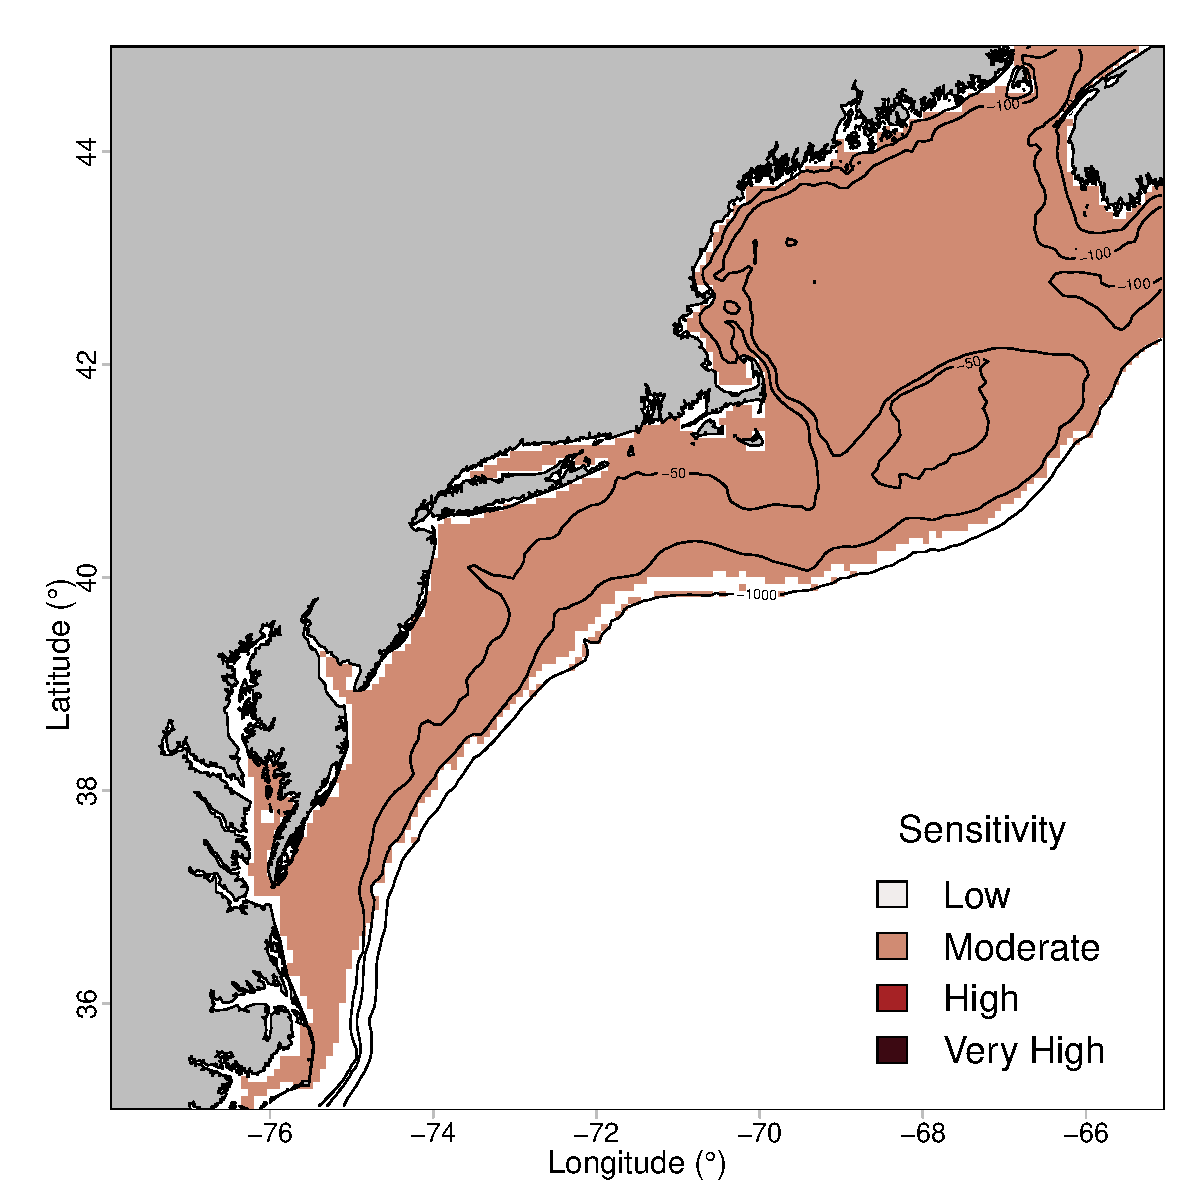
\includegraphics[width=0.85\textwidth,height=\textheight]{../figures/Atlantic herring/Atlanticherring_sensitivity_2.0.pdf}

}

\caption{\label{fig-sens-herring}Atlantic herring Sensitivity on the
Northeast Shelf}

\end{figure}%

Atlantic herring had a \textbf{Moderate} sensitivity score, with a
certainty of 90\%. This score was driven by two attributes: Stock Size
(4) and Spawning Cycle (2.8) (\textbf{?@fig-sum-tab-herring}).

Spawning success and recruitment is highly correlated with temperatures.
The optimal spawning temperature window has shortened over the past 30
years (Kanwit and Libby 2009; Molina 2025). Mismatches between larvae
and prey abundance lead to higher mortality (Randall et al. 2022). As of
the 2024 assessment, herring are overfished but not experiencing
overfishing (Northeast Fisheries Science Center (NEFSC) 2024).

In the previous assessment, herring received a Low sensitivity score.
This score was driven by Early Life History Requirements, citing the
need for demersal spawning habitat (Hare et al. 2016).

\subsubsection{Exposure:}\label{exposure}

\begin{figure}[H]

\centering{

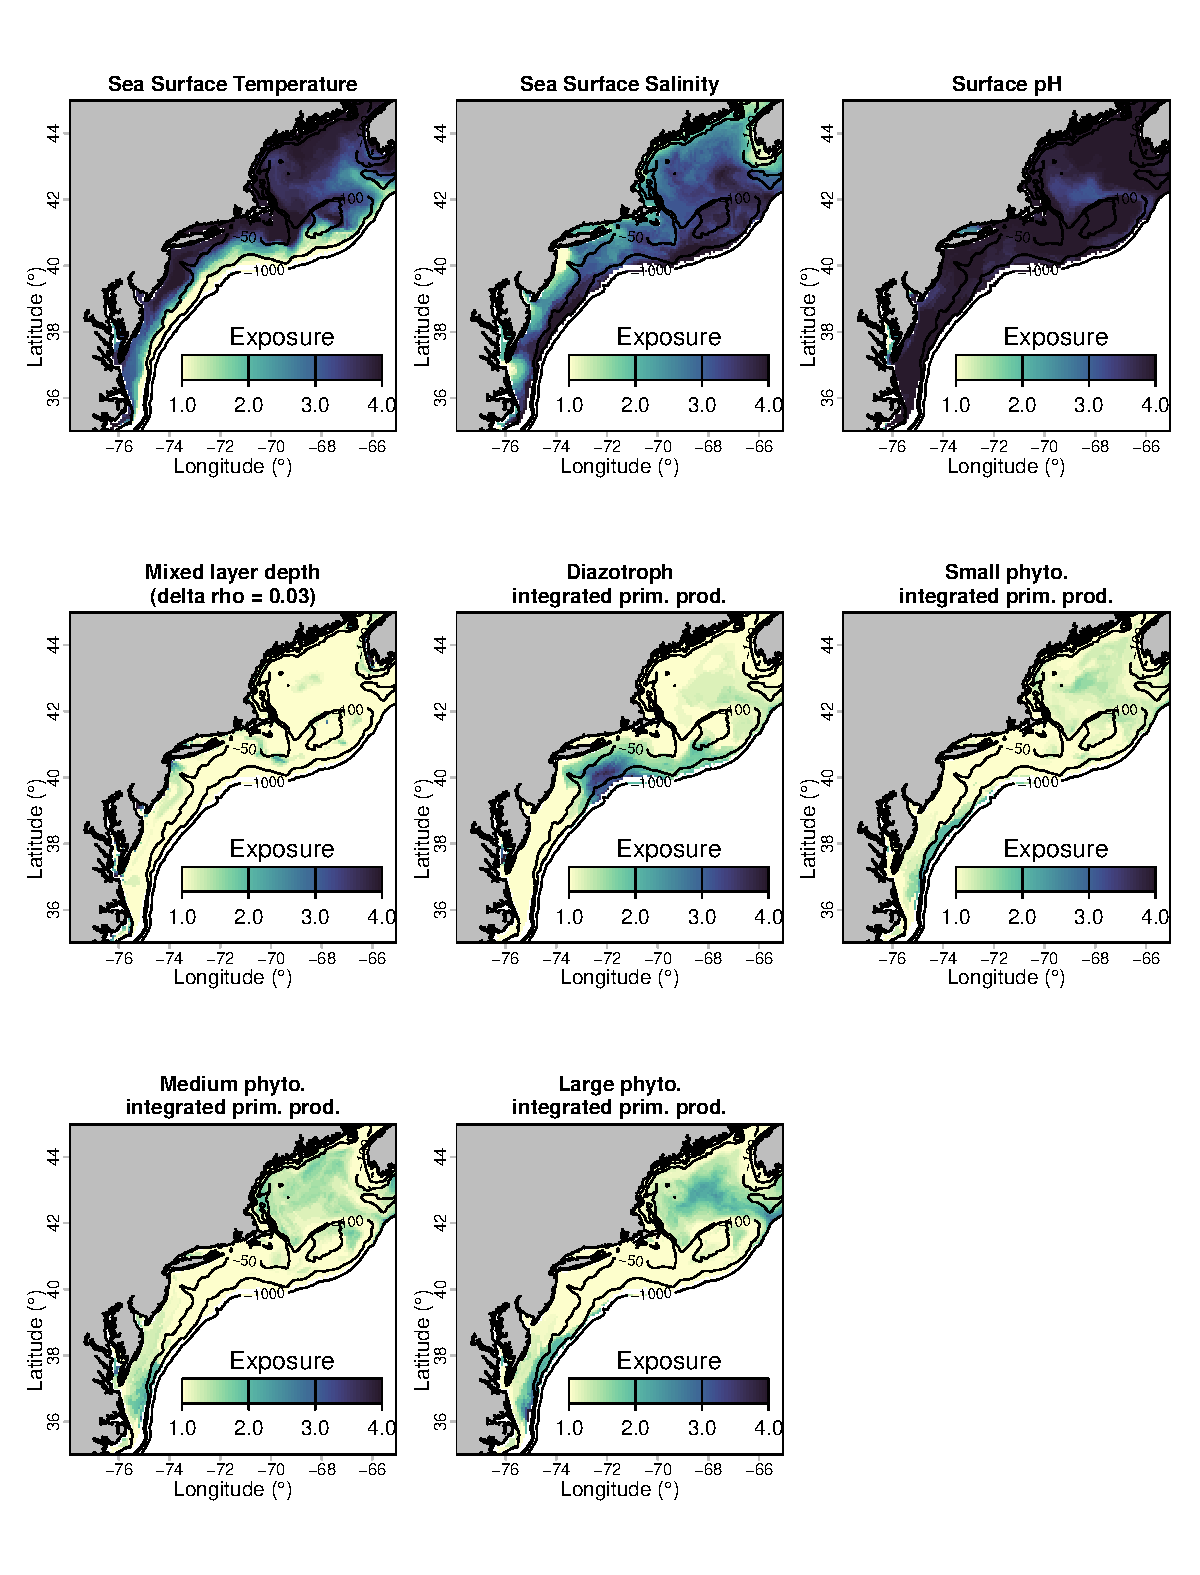
\includegraphics[width=0.85\textwidth,height=\textheight]{../figures/Atlantic herring/variable_exposure_maps_r20250925_i202501_r20250715_20142023.pdf}

}

\caption{\label{fig-fact-exp-herring}Maps of each Exposure Factor for
Atlantic herring. Exposure was calculated between 2014-2023 and
2025-2035}

\end{figure}%

Mean total exposure for Atlantic herring was \textbf{High} (2.97 +/-
0.32) (\textbf{?@fig-sum-tab-herring}). Exposure was uniform across the
continental shelf, with Very High exposure on Georges Bank, and Low to
Moderate Exposure south of Cape Cod and east of the Chesapeake Bay
(Figure~\ref{fig-exp-herring}). These patterns were driven by very high
exposure due to sea surface temperature, salinity, and pH
(Figure~\ref{fig-fact-exp-herring}).

In the previous Assessment, Atlantic Herring also received a High
exposure score, driven by surface temperatures and ocean acidification
(Hare et al. 2016).

\begin{figure}[H]

\centering{

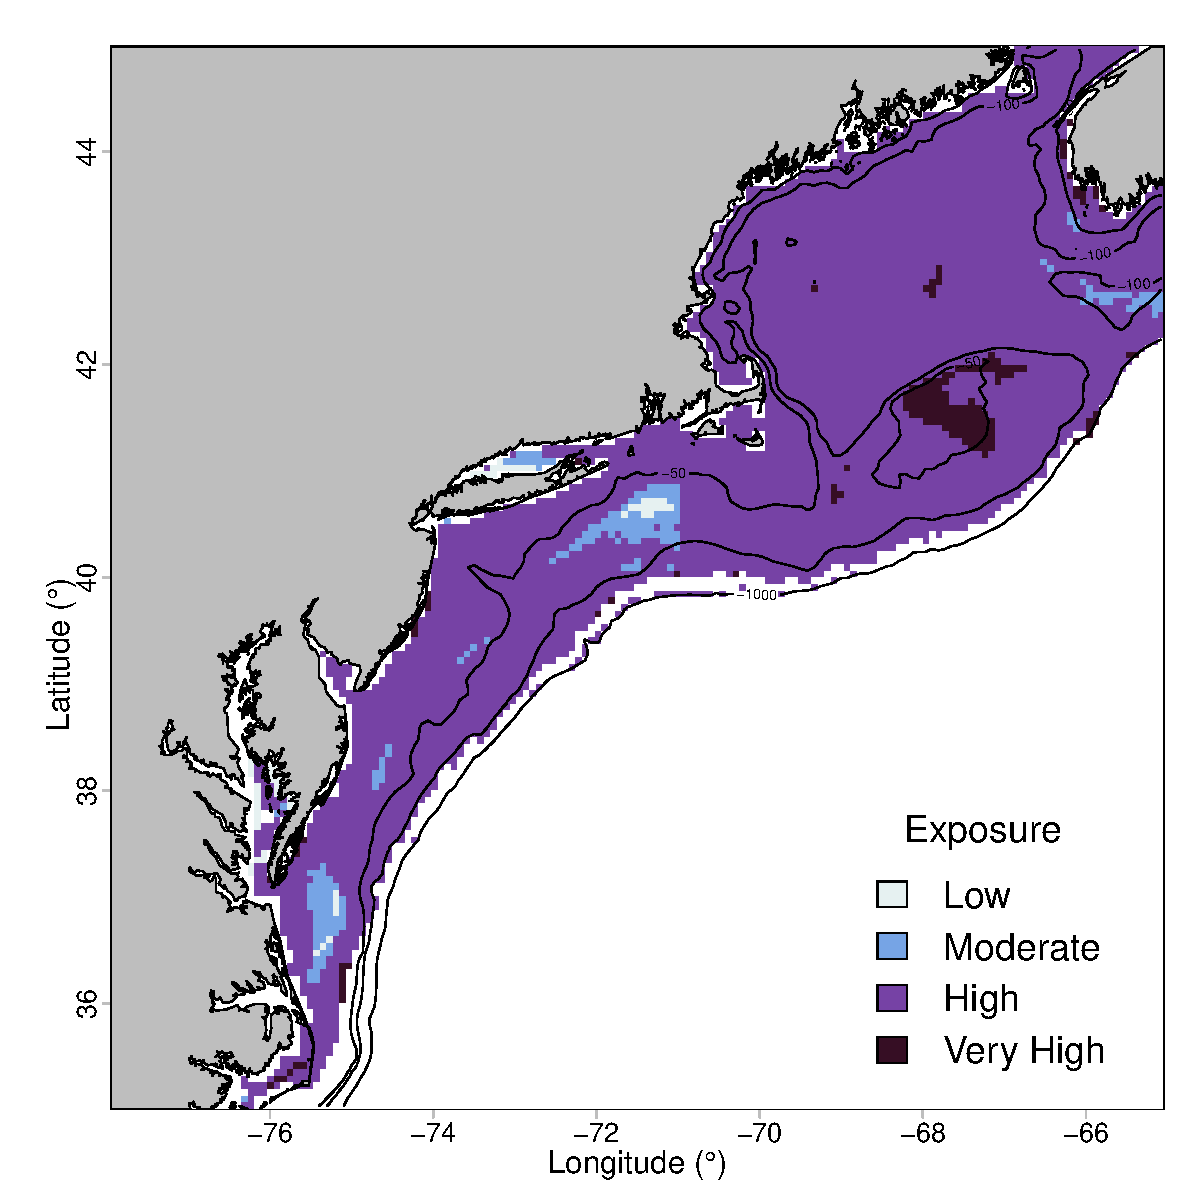
\includegraphics[width=0.85\textwidth,height=\textheight]{../figures/Atlantic herring/total_exposure_map_only_all_var_r20250925_i202501_r20250715_20142023.pdf}

}

\caption{\label{fig-exp-herring}Total Exposure on the Northeast Shelf
for Atlantic herring. Total Exposure is calculated by applying the logic
rule from Hare et al. (2016) within grid cells across exposure factors
(see Figure~\ref{fig-fact-exp-herring})}

\end{figure}%

\subsubsection{Vulnerability:}\label{vulnerability}

\begin{figure}[H]

\centering{

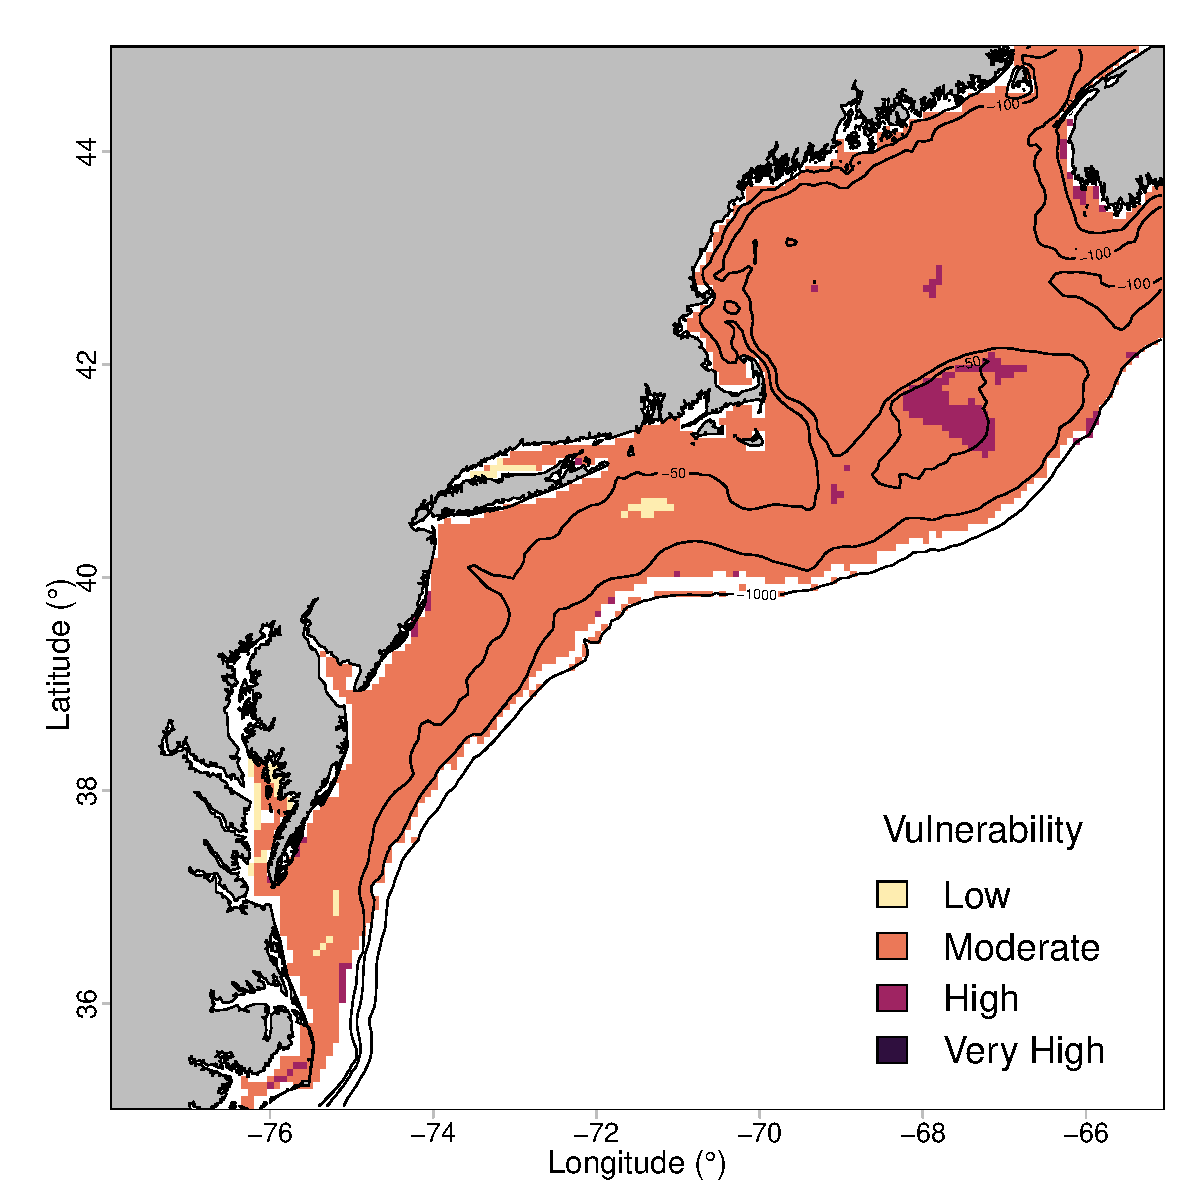
\includegraphics[width=0.85\textwidth,height=\textheight]{../figures/Atlantic herring/total_vulnerability_map_only_all_var_r20250925_i202501_r20250715_20142023.pdf}

}

\caption{\label{fig-vuln-herring}Vulnerability on the Northeast Shelf
for Atlantic herring. Vulnerability is the product of sensitivity and
exposure (see Figure~\ref{fig-exp-herring} and
Figure~\ref{fig-sens-herring})}

\end{figure}%

Mean Vulnerability for Atlantic Herring was \textbf{Moderate} (5.95 +/-
0.64) (\textbf{?@fig-sum-tab-herring}). Vulnerability was uniform across
the shelf when all factors were considered, with peaks of High
Vulnerability off Georges Bank (Figure~\ref{fig-vuln-herring}).

In the previous Assessment, Herring received a Low Vulnerability Score.
The change in this assessment is due to an increase in the Sensitivity
Score (Hare et al. 2016).

\subsection{Data Quality Metrics}\label{data-quality-metrics}

\subsubsection{Life History Data
Quality:}\label{life-history-data-quality}

95\% of data quality scores were greater than or equal to 2, indicating
excellent data quality. No data gaps (mean attribute data quality score
\textless{} 2) were identified for this species
(\textbf{?@fig-sum-tab-herring}).

\subsubsection{Model Confidence Score:}\label{model-confidence-score}

The herring ensemble model received a model confidence score of 1.6 (+/-
0.3), indicating low confidence in the model. While the model results
represented general distribution patterns, experts noted that residuals
(differences between observed and predicted values) were high in March
and September. This was likely due to herring catchability in the
surveys and interannual variability in migration timing. The ensemble
model's AUC was 0.73, indicating fair performance.

\subsection{Additional Metrics}\label{additional-metrics}

\subsubsection{Distribution Shifts:}\label{distribution-shifts}

\begin{figure}[H]

\centering{

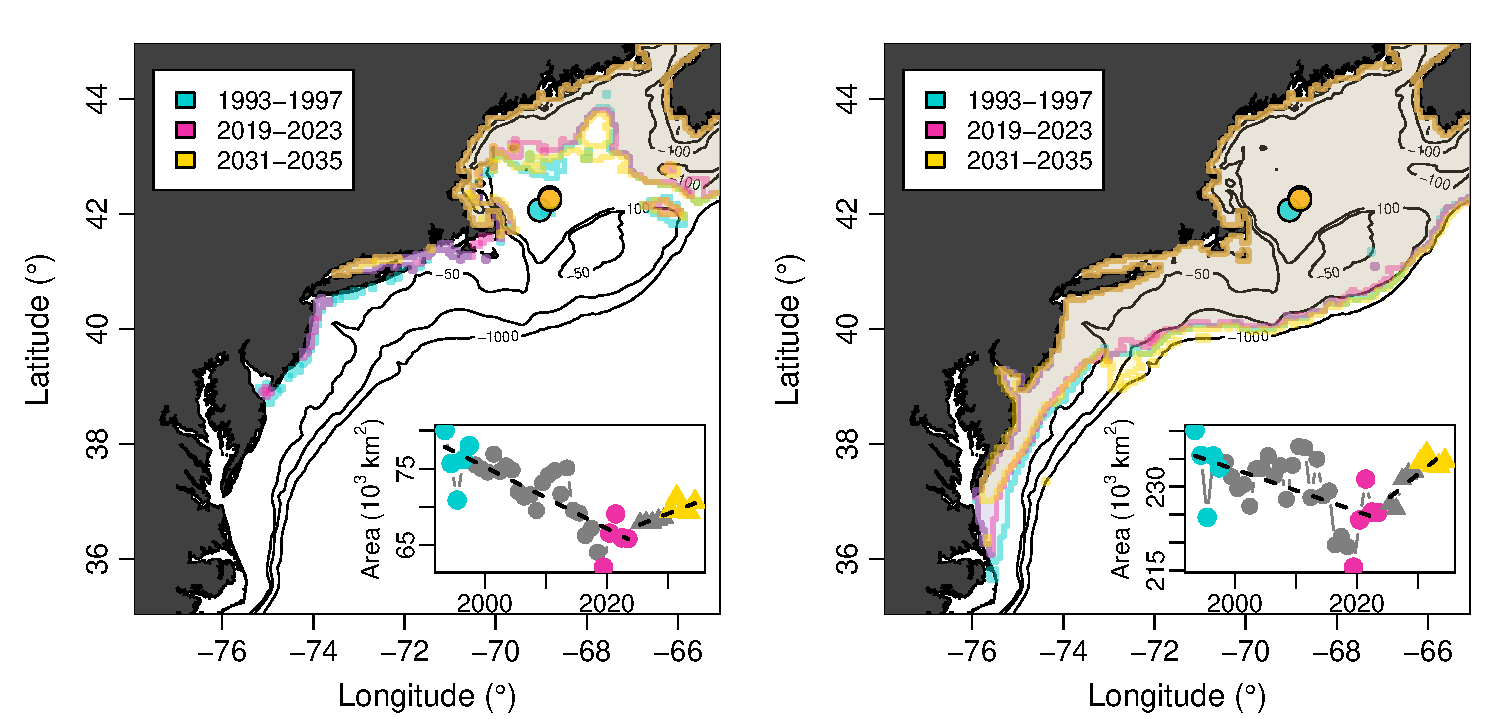
\includegraphics[width=0.85\textwidth,height=\textheight]{../figures/Atlantic herring/distribution_shifts_static_r20250715_r20250925_i202501.pdf}

}

\caption{\label{fig-shifts-herring}Distribution shifts on the Northeast
Shelf for Atlantic herring. Polygons illustrate core habitat (left) and
species range (right) for five-year average periods. Points illustrate
weighted centroid, calculated as the average position with species
distribution models as weights. Inset timeseries illustrate the shift in
core and habitat range area over time. Circles represent points from the
MOM6 hindcast; triangles represent points from the MOM6 forecast. Dashed
lines represent significant linear regressions}

\end{figure}%

\emph{Note: For an animated version of this plot, please see the online
version of this document.}

The weighted distribution centroid for Atlantic herring has shifted
northward by 30 km since 1993. This is due to the northward shift of the
southern edges of herring core habitat and their entire range. As a
result, herring habitat area has declined significantly between 1993 and
2023 (Figure~\ref{fig-shifts-herring}).

However, herring habitats are predicted to expand slightly in the next
decade. Habitat areas are expected to significantly increase between
2025 and 2035. Core habitat in the Gulf of Maine is predicted to expand
southward, resulting in a nearly 4 km southward shift in the predicted
distribution weighted centroid (Figure~\ref{fig-shifts-herring}).

Herring received a High Distributional Vulnerability Rank in the
previous assessment due to high mobility and larval duration (Hare et
al. 2016).

\begin{longtable}[]{@{}
  >{\raggedright\arraybackslash}p{(\columnwidth - 10\tabcolsep) * \real{0.1667}}
  >{\raggedright\arraybackslash}p{(\columnwidth - 10\tabcolsep) * \real{0.1667}}
  >{\raggedright\arraybackslash}p{(\columnwidth - 10\tabcolsep) * \real{0.1667}}
  >{\raggedright\arraybackslash}p{(\columnwidth - 10\tabcolsep) * \real{0.1667}}
  >{\raggedright\arraybackslash}p{(\columnwidth - 10\tabcolsep) * \real{0.1667}}
  >{\raggedright\arraybackslash}p{(\columnwidth - 10\tabcolsep) * \real{0.1667}}@{}}
\caption{Distribution shifts based on five-year average distributions.
Changes are calculated relative to the previous time
period.}\tabularnewline
\toprule\noalign{}
\begin{minipage}[b]{\linewidth}\raggedright
Time Period
\end{minipage} & \begin{minipage}[b]{\linewidth}\raggedright
Weighted Centroid Shift (km \& bearing)
\end{minipage} & \begin{minipage}[b]{\linewidth}\raggedright
Core Habitat Area (change) (km\textsuperscript{2})
\end{minipage} & \begin{minipage}[b]{\linewidth}\raggedright
Habitat Total Area (change) (km\textsuperscript{2})
\end{minipage} & \begin{minipage}[b]{\linewidth}\raggedright
Latitude Range (change) (deg)
\end{minipage} & \begin{minipage}[b]{\linewidth}\raggedright
Change in Longitude Range (deg)
\end{minipage} \\
\midrule\noalign{}
\endfirsthead
\toprule\noalign{}
\begin{minipage}[b]{\linewidth}\raggedright
Time Period
\end{minipage} & \begin{minipage}[b]{\linewidth}\raggedright
Weighted Centroid Shift (km \& bearing)
\end{minipage} & \begin{minipage}[b]{\linewidth}\raggedright
Core Habitat Area (change) (km\textsuperscript{2})
\end{minipage} & \begin{minipage}[b]{\linewidth}\raggedright
Habitat Total Area (change) (km\textsuperscript{2})
\end{minipage} & \begin{minipage}[b]{\linewidth}\raggedright
Latitude Range (change) (deg)
\end{minipage} & \begin{minipage}[b]{\linewidth}\raggedright
Change in Longitude Range (deg)
\end{minipage} \\
\midrule\noalign{}
\endhead
\bottomrule\noalign{}
\endlastfoot
1993-1997 & NA & 76,345 & 234,718 & 6.11 & 9.1 \\
2019-2023 & 30.3 km NE & 65,973 (-10,372) & 224,811 (-9,907) & 5.67
(-0.44) & 8.82 (-0.32) \\
2031-2035 & 3.7 km S & 70,052 (+4,078) & 234,504 (+9,693) & 5.74 (+0.06)
& 8.65 (-0.16) \\
\end{longtable}

\subsubsection{Directional Effect:}\label{directional-effect}

Herring are very likely to be \textbf{negatively} impacted by future
climate change along the Northeast Shelf (100\% certainty in expert
scores). Warming temperatures and increasing bottom salinities are
decreasing the amount of favorable habitat for herring (Suca et al.
2021). Mismatches between larvae and prey abundances have resulted in
slower growth and higher larval mortality (Randall et al. 2022). The
2016 Climate Vulnerability Assessment for the Northeast Shelf also
suggested that herring would be negatively impacted, but with more
uncertainty (Hare et al. 2016).

\subsection{Climate Effects on Abundance and
Distribution}\label{climate-effects-on-abundance-and-distribution}

A number of Atlantic herring life history parameters are linked to
drivers of climate change. Climate-related mismatches between Atlantic
herring larval feeding and prey abundance have resulted in slower growth
and higher mortality (Randall et al. 2022). J. P. Gröger, Kruse, and
Rohlf (2010) found that lags in the North Atlantic Oscillation (NAO) and
Atlantic Multi-decadal Oscillation (AMO) were the primary drivers of
Atlantic herring recruitment. Winter NAO has also indirectly influenced
recruitment in multiple herring stocks (Axenrot and Hansson 2003;
Oskarsson and Taggart 2010; Lynam et al. 2005) and may be used to
predict recruitment with lead times up to 5 years (J. P. Gröger, Kruse,
and Rohlf 2010). Atlantic herring recruitment is also influenced by
larval temperatures, the Gulf Stream Index, and food availability from
water mass movement (Molina 2025). Favorable habitat for Atlantic
herring in the Northwest Atlantic is currently decreasing with rising
temperatures and bottom salinity (Suca et al. 2021), with herring
populations in warmer waters responding more negatively to increasing
temperatures than those in colder waters (Beaudry-Sylvestre, Benoît, and
Hutchings 2024). Herring larvae in the Baltic Sea are facing more heat
stress and cardiac dysfunction with an increase in the number of marine
heat waves (M. Gröger et al. 2024). Migration and distribution of
Atlantic herring is also linked with thermal oceanic fronts between
colder, less saline continental shelf water and warmer, more salient
slope water (where plankton are also usually more abundant) (Kelly and
Moring 1986).

\subsection{Life History Synopsis}\label{life-history-synopsis}

Atlantic herring in the Northwest Atlantic reside from southern Labrador
in Canada to Cape Hatteras, NC (Stevenson and Scott 2005). They spawn
primarily on Jeffreys Ledge and Georges Bank between July and November,
with peaks in August - September in the Gulf of Maine. However, recent
research has suggested that the optimal spawning temperature window has
shortened over the past 30 years (Kanwit and Libby 2009; Molina 2025).
Early life history development is inversely related to water
temperature, with slower growth occurring at higher temperatures
(Stevenson and Scott 2005). Eggs hatch after 6-15 days, and larval
development time ranges from 4-8 months. Larvae absorb their yolk sac
within 2.5 - 6 days, at which point the larvae become pelagic and can be
transported away from or retained near spawning habitats, depending on
prevailing current systems (Lough and Cohen 1982). Predation of eggs is
linked to high mortality. Predators include haddock, cod, mackerel,
winter flounder, moon snails, hermit crabs and starfish. Strong haddock
recruitment has been linked to low abundances of larval herring (Boyar
et al. 1973; Burbank et al. 2023). Larval herring prey on copepods, with
size depending on the size of the larvae (Sherman and Honey 1971).
Juveniles form large schools in coastal waters (i.e.~estuaries and
embayments) throughout the Gulf of Maine in the spring and summer, and
overwinter in deep bays or offshore (Stevenson and Scott 2005).
Juveniles and adults are planktivorous and opportunistic feeders. As
they grow and the size of their jaws increases, they consume larger
organisms. Their diet therefore varies with season, their age and size,
and location. (Stevenson and Scott 2005; Sherman and Perkins 1971). A
lack of availability of preferred prey in adults (due to strong mixing
in the water column) can lead to suboptimal feeding and slow growth
resulting in increased mortality from starvation and predation
(Stevenson and Scott 2005). Adult herring make extensive seasonal
migrations between summer spawning grounds on Georges Bank and in the
Gulf of Maine and overwintering areas in southern New England and the
Mid-Atlantic region (Stevenson and Scott 2005). There are two major
spawning stocks in the Northwest Atlantic: the Gulf of Maine and Georges
Bank/Nantucket Shoals. Stocks are separated based on larval distribution
patterns, spawning times/locations, and growth rates (Iles and Sinclair
1982; Boyar et al. 1973; Anthony and Waring 1980). Both stocks are
currently assessed in the U.S. as a single coastal stock complex managed
by the New England Fishery Management Council. As of the most recent
assessment (Northeast Fisheries Science Center (NEFSC) 2024), the stock
is overfished but not experiencing overfishing based on the biological
reference points for spawning stock biomass (SSB) and fishing mortality
(F).

\subsection{Supplemental Scores}\label{supplemental-scores}

\subsubsection{Exposure Timeseries}\label{exposure-timeseries}

\begin{figure}[H]

\centering{

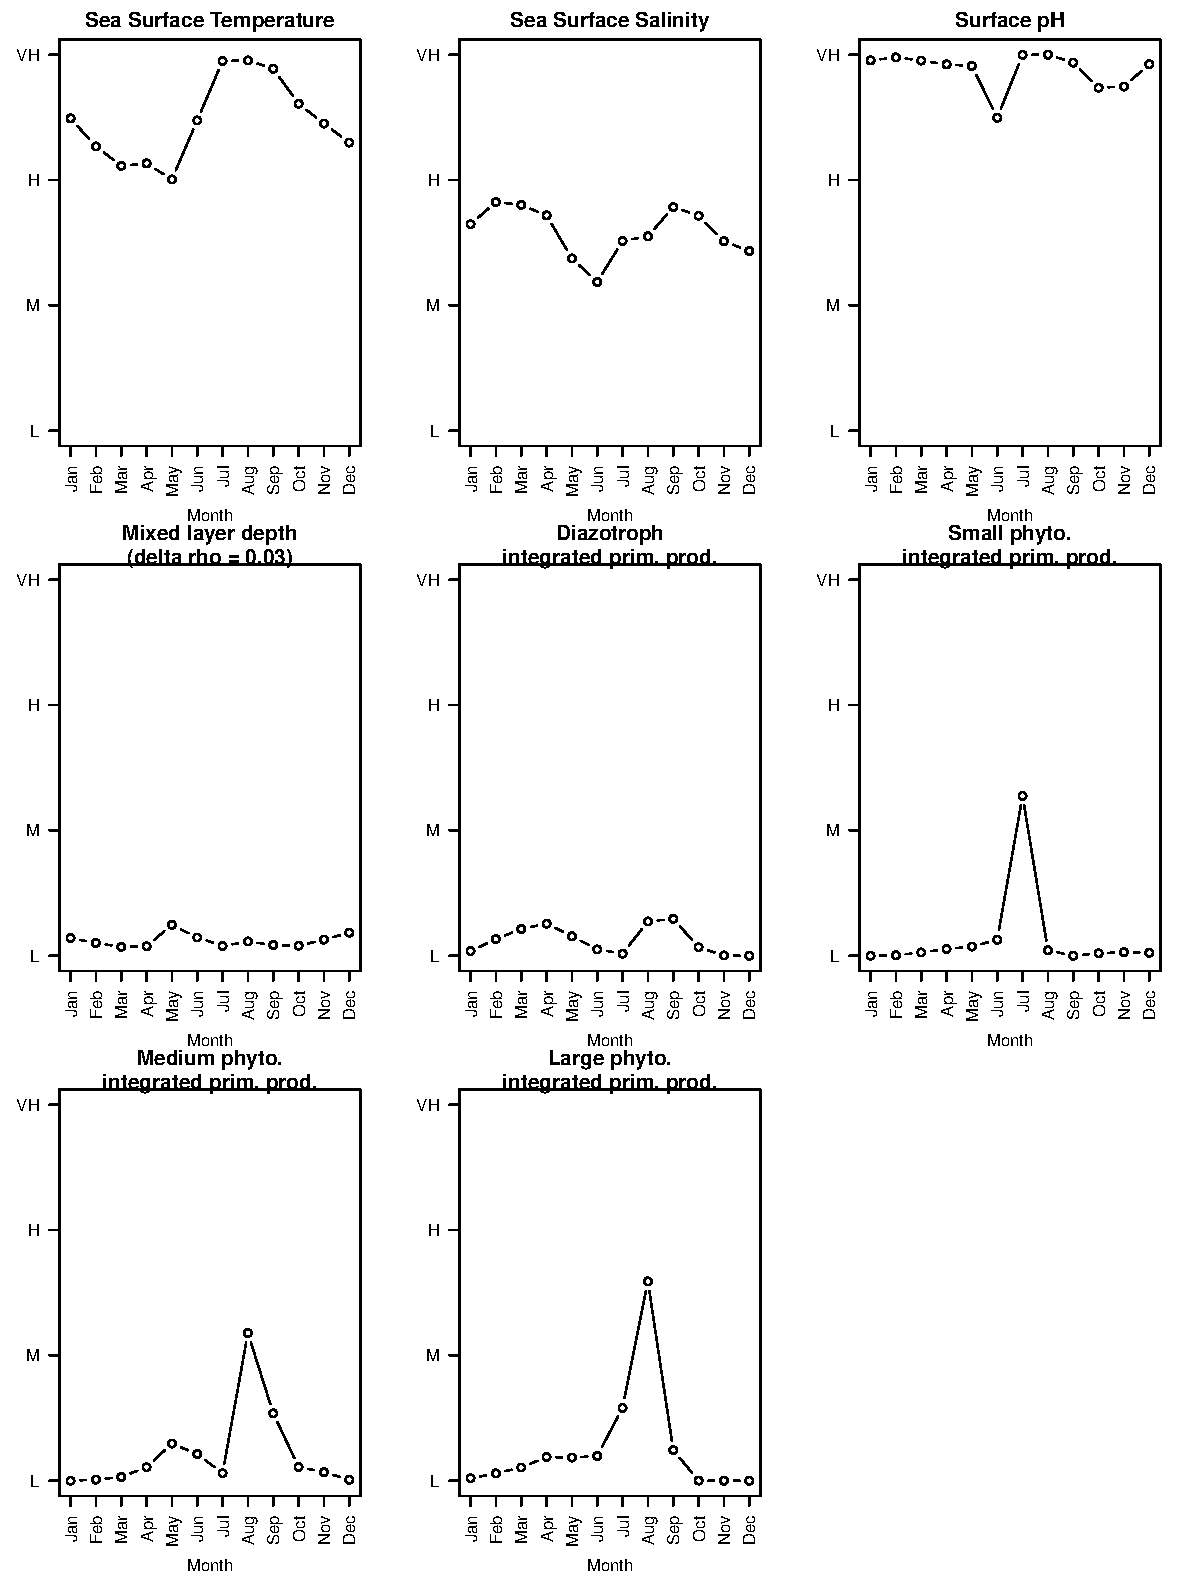
\includegraphics[width=0.85\textwidth,height=\textheight]{../figures/Atlantic herring/variable_exposure_timeseries_r20250925_i202501_r20250715_20142023.pdf}

}

\caption{\label{fig-exp-month-tm-herring}Monthly Timeseries of each
Exposure Factor for Atlantic herring. Exposure was calculated between
2014-2023 and 2025-2035}

\end{figure}%

Monthly exposure was consistently High. There was no variation across
months (Figure~\ref{fig-exp-month-herring};
Figure~\ref{fig-exp-month-tm-herring}).

\begin{figure}[H]

\centering{

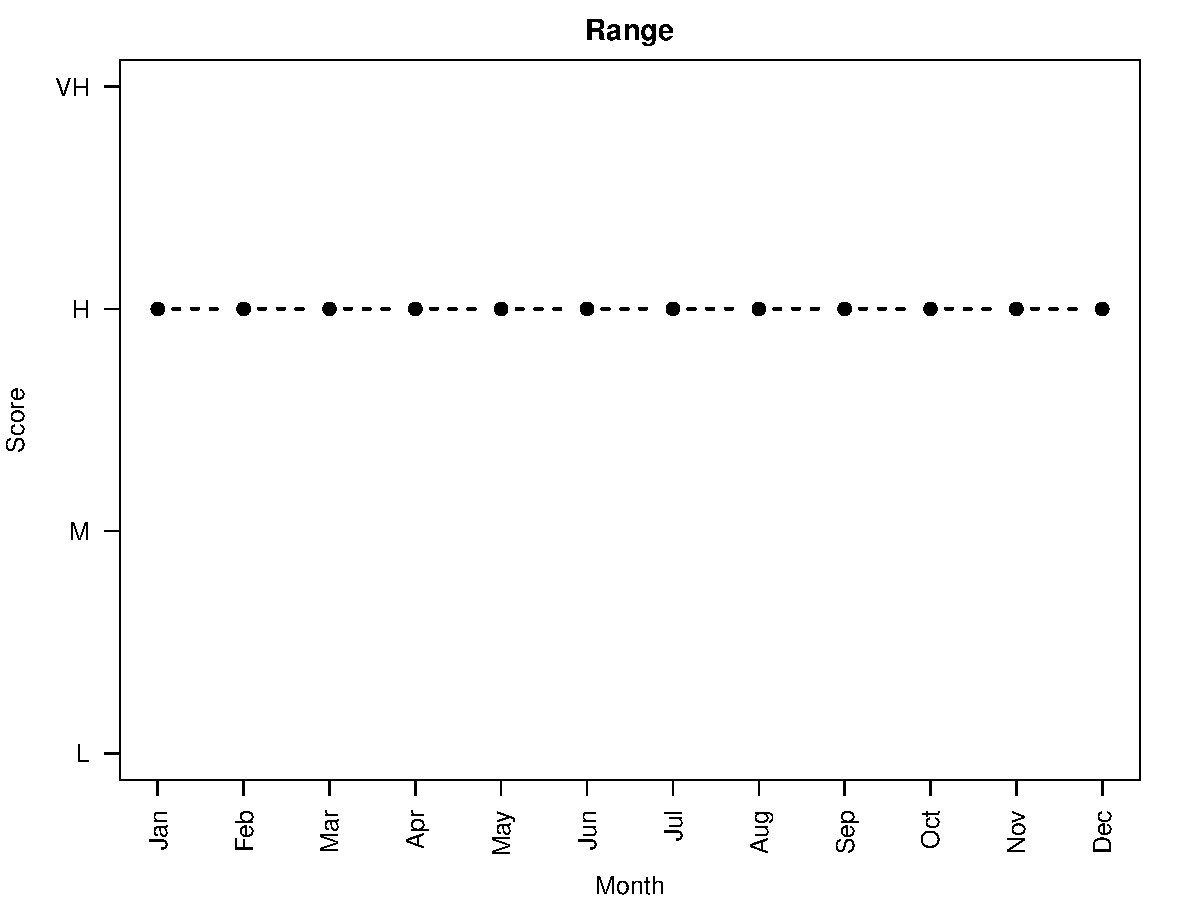
\includegraphics[width=0.85\textwidth,height=\textheight]{../figures/Atlantic herring/total_exposure_timeseries_only_all_var_r20250925_i202501_r20250715_20142023.pdf}

}

\caption{\label{fig-exp-month-herring}Timeseries of Total Exposure for
Atlantic herring}

\end{figure}%

\subsubsection{Exposure due to Significant
Factors}\label{exposure-due-to-significant-factors}

\begin{figure}[H]

\centering{

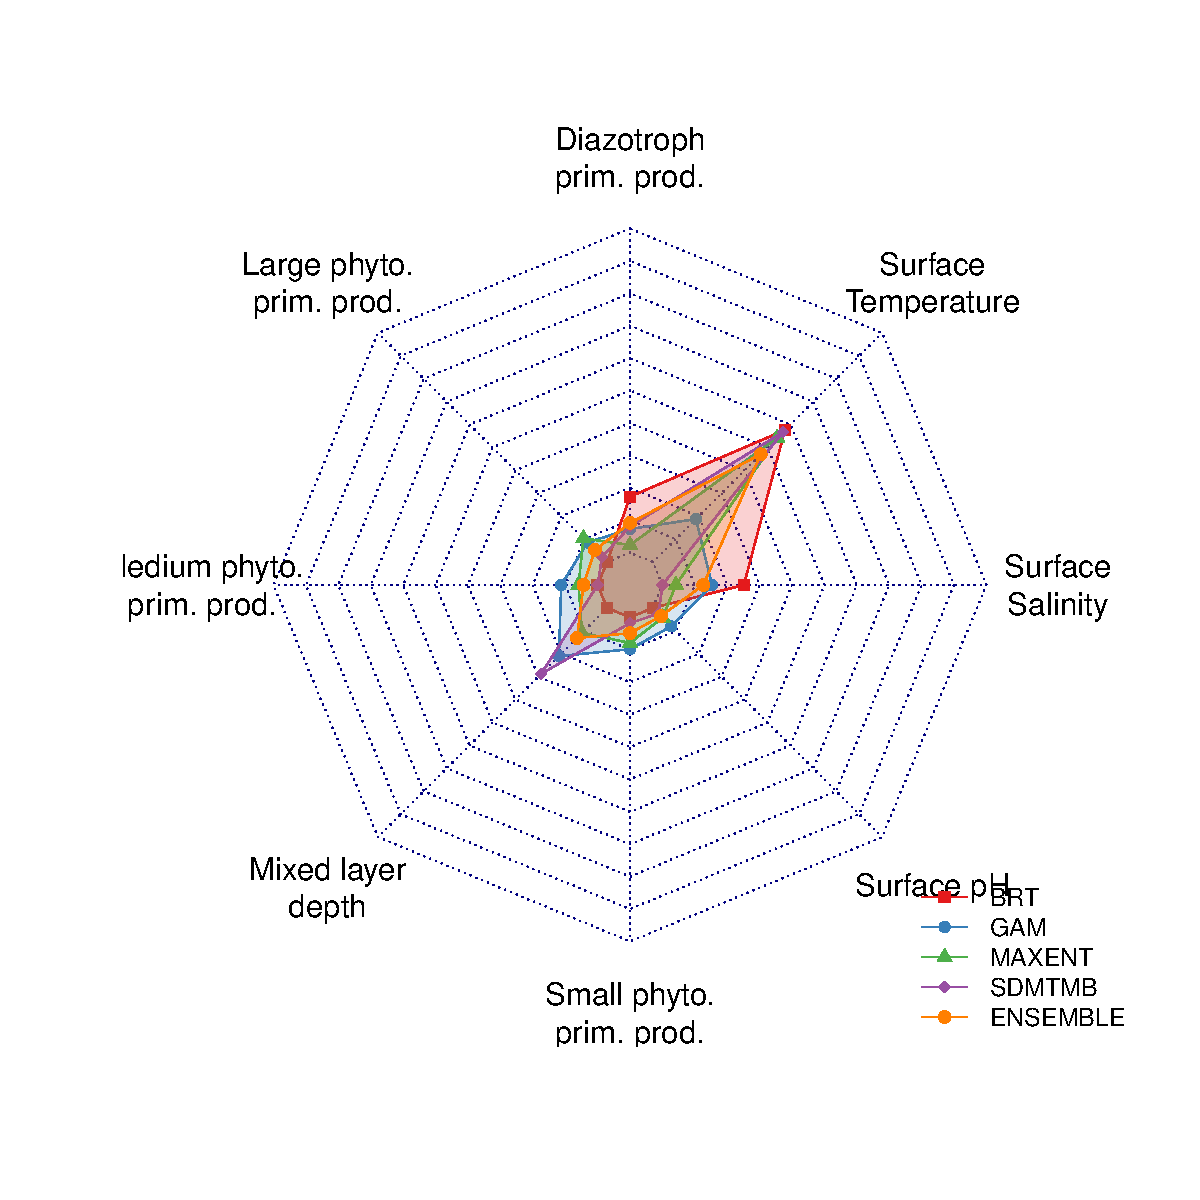
\includegraphics[width=0.85\textwidth,height=\textheight]{../figures/Atlantic herring/dynamic_variable_importance_r20250715.pdf}

}

\caption{\label{fig-radar-herring}Dynamic Factors driving Atlantic
herring distributions. The closer the polygon is to the edge of the
figure, the more important the variable is. Each ring represents 10\%
variance explained. Factors must explain at least 10\% of variance in
the ensemble model to be used to calculate total exposure.}

\end{figure}%

Sea surface temperature, surface salinity, and mixed layer depth were
all important drivers of herring distributions
(Figure~\ref{fig-radar-herring}). Temperature and salinity have been
linked to favorable habitats for herring (Suca et al. 2021) and
increased mixing has been linked to decreased prey availability and
increased mortality (Stevenson and Scott 2005). When these factors alone
were used to calculate exposure, mean Exposure dropped to Moderate (1.72
+/- 0.83) (Figure~\ref{fig-exp-imp-herring}). Exposure due to these
variables was greatest in the Gulf of Maine and in the middle of the
continental shelf (\textbf{?@fig-sum-imp-herring}).

\begin{figure}[H]

\centering{

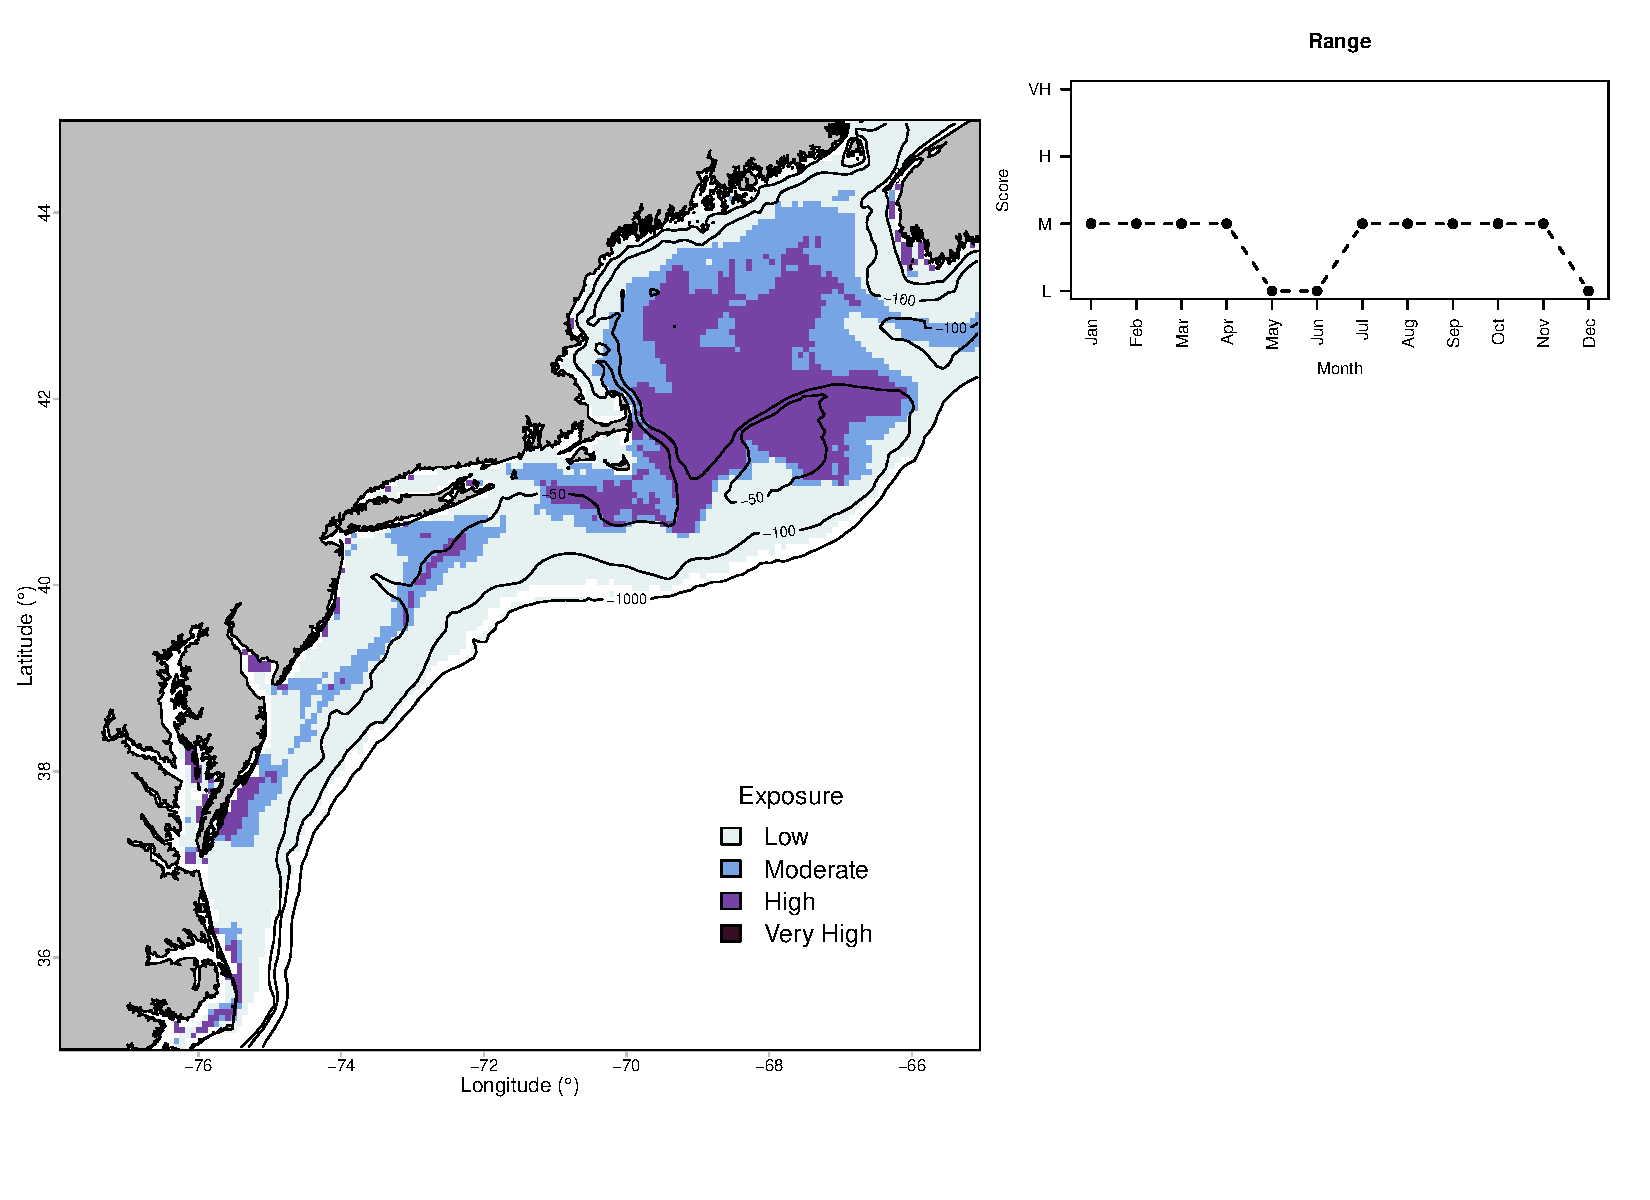
\includegraphics[width=0.85\textwidth,height=\textheight]{../figures/Atlantic herring/total_exposure_map_timeseries_imp_var_r20250925_i202501_r20250715_20142023.pdf}

}

\caption{\label{fig-exp-imp-herring}Total Exposure Map and Timeseries
when Exposure was calculated with only Exposure Factors critical to
Atlantic herring distributions}

\end{figure}%

\subsection*{References}\label{references}
\addcontentsline{toc}{subsection}{References}

\phantomsection\label{refs}
\begin{CSLReferences}{1}{0}
\bibitem[\citeproctext]{ref-Anthony1980}
Anthony, V. C., and G. T. Waring. 1980. {``Estimates of Herring Spawning
Stock Biomass and Egg Production for the Georges Bank-Gulf of Maine
Region.''} Res. Doc. 80/IX/135. Northwest Atl. Fish. Organ. (NAFO) Sci.
Counc.

\bibitem[\citeproctext]{ref-Axenrot2003}
Axenrot, T., and S. Hansson. 2003. {``Predicting Herring Recruitment
from Young‐of‐the‐year Densities, Spawning Stock Biomass, and
Climate.''} \emph{Limnology and Oceanography} 48 (4): 1716--20.

\bibitem[\citeproctext]{ref-Beaudry2024}
Beaudry-Sylvestre, M., H. P. Benoît, and J. A. Hutchings. 2024.
{``Coherent Long-Term Body-Size Responses Across All Northwest Atlantic
Herring Populations to Warming and Environmental Change Despite
Contrasting Harvest and Ecological Factors.''} \emph{Global Change
Biology} 30: e17187. \url{https://doi.org/10.1111/gcb.17187}.

\bibitem[\citeproctext]{ref-Boyar1973}
Boyar, H. C., R. R. Marak, F. E. Perkins, and R. A. Clifford. 1973.
{``Seasonal Distribution and Growth of Larval Herring (Clupea Harengus
l.) in the Georges Bank -- Gulf of Maine Area from 1962 to 1970.''}
\emph{J. Cons. Int. Explor. Mer} 35: 36--51.

\bibitem[\citeproctext]{ref-Burbank2023}
Burbank, J., J. L. McDermid, F. Turcotte, and N. Rolland. 2023.
{``Temporal Variation in von Bertalanffy Growth Curves and Generation
Time of Southern Gulf of St. Lawrence Spring and Fall Spawning Atlantic
Herring (Clupea Harengus).''} \emph{Fishes} 8: 205.
\url{https://doi.org/10.3390/fishes8040205}.

\bibitem[\citeproctext]{ref-Groger2010}
Gröger, J. P., G. H. Kruse, and N. Rohlf. 2010. {``Slave to the Rhythm:
How Large-Scale Climate Cycles Trigger Herring (Clupea Harengus)
Regeneration in the North Sea.''} \emph{ICES Journal of Marine Science}
67 (3): 454--65.

\bibitem[\citeproctext]{ref-Groger2024}
Gröger, M., F. Börgel, S. Karsten, H. E. M. Meier, K. Safonova, C.
Dutheil, A. Receveur, and P. Polte. 2024. {``Future Climate Change and
Marine Heatwaves - Projected Impact on Key Habitats for Herring
Reproduction.''} \emph{Science of the Total Environment} 951: 175756.
\url{https://doi.org/10.1016/j.scitotenv.2024.175756}.

\bibitem[\citeproctext]{ref-hare2016vulnerability}
Hare, Jonathan A, Wendy E Morrison, Mark W Nelson, Megan M Stachura,
Eric J Teeters, Roger B Griffis, Michael A Alexander, et al. 2016. {``A
Vulnerability Assessment of Fish and Invertebrates to Climate Change on
the Northeast US Continental Shelf.''} \emph{PloS One} 11 (2): e0146756.

\bibitem[\citeproctext]{ref-Iles1982}
Iles, T. D., and M. Sinclair. 1982. {``Atlantic Herring Stock
Discreteness and Abundance.''} \emph{Science} 215: 627--33.

\bibitem[\citeproctext]{ref-Kanwit2009}
Kanwit, J. K., and D. A. Libby. 2009. {``Seasonal Movements of Atlantic
Herring (Clupea Harengus): Results from a Four Year Tagging Study
Conducted in the Gulf of Maine and Southern New England.''}
\emph{Journal of Northwest Atlantic Fishery Science} 40: 29--39.
\url{https://doi.org/10.2960/j.v40.m577}.

\bibitem[\citeproctext]{ref-Kelly1986}
Kelly, K. H., and J. R. Moring. 1986. {``Species Profiles: Life
Histories and Environmental Requirements of Coastal Fishes and
Invertebrates (North Atlantic) - Atlantic Herring.''} Biol. Rep. 82
(11.38). U.S. Fish Wildl. Serv.

\bibitem[\citeproctext]{ref-Lough1982}
Lough, R. G., and R. E. Cohen. 1982. {``Vertical Distribution of
Recently-Hatched Herring Larvae and Associated Zooplankton on Jeffreys
Ledge and Georges Bank, October 1974.''} Ref. Doc. 82-10. U.S. Natl.
Mar. Fish. Serv. Northeast Fish. Cent. Woods Hole Lab.

\bibitem[\citeproctext]{ref-Lynam2005}
Lynam, C. P., M. R. Heath, S. J. Hay, and A. S. Brierley. 2005.
{``Evidence for Impacts by Jellyfish on North Sea Herring
Recruitment.''} \emph{Marine Ecology Progress Series} 298: 157--67.

\bibitem[\citeproctext]{ref-Molina2025}
Molina, A. 2025. {``Atlantic Herring Ecosystem and Socioeconomic
Profile.''}
\url{https://repository.library.noaa.gov/view/noaa/71713/noaa_71713_DS1.pdf}.

\bibitem[\citeproctext]{ref-NEFSC2024_herring}
Northeast Fisheries Science Center (NEFSC). 2024. {``Atlantic Herring
2024 Management Track Assessment Report.''} NOAA Fisheries.
\url{https://d23h0vhsm26o6d.cloudfront.net/4.c_Atlantic_Herring_2024-Management-Track-Stock-Assessment-Report.pdf}.

\bibitem[\citeproctext]{ref-Oskarsson2010}
Oskarsson, G. J., and C. T. Taggart. 2010. {``Variation in Reproductive
Potential and Influence on Icelandic Herring Recruitment.''}
\emph{Fisheries Oceanography} 19 (5): 412--26.

\bibitem[\citeproctext]{ref-Randall2022}
Randall, J. R., H. M. Murphy, D. Robert, and M. Geoffroy. 2022.
{``Forage Fish as a Predator: Summer and Autumn Diet of Atlantic Herring
in Trinity Bay, Newfoundland.''} \emph{Fisheries Research} 252: 106331.
\url{https://doi.org/10.1016/j.fishres.2022.106331}.

\bibitem[\citeproctext]{ref-Sherman1971_larval}
Sherman, K., and K. A. Honey. 1971. {``Seasonal Variations in the Food
of Larval Herring in Coastal Waters of Maine.''} \emph{Rapp. P.-V. Réun.
Cons. Int. Explor. Mer} 160: 121--24.

\bibitem[\citeproctext]{ref-Sherman1971_juvenile}
Sherman, K., and H. C. Perkins. 1971. {``Seasonal Variation in the Food
of Juvenile Herring in Coastal Waters of Maine.''} \emph{Trans. Am.
Fish. Soc.} 100: 121--24.

\bibitem[\citeproctext]{ref-Stevenson2005}
Stevenson, D. K., and M. L. Scott. 2005. {``Essential Fish Habitat
Source Document: Atlantic Herring, Clupea Harengus, Life History and
Habitat Characteristics.''} NOAA Technical Memorandum NMFS-NE-192.

\bibitem[\citeproctext]{ref-Suca2021}
Suca, J. J., J. J. Deroba, D. E. Richardson, R. Ji, and J. K. Llopiz.
2021. {``Environmental Drivers and Trends in Forage Fish Occupancy of
the Northeast US Shelf.''} \emph{ICES Journal of Marine Science} 78
(10): 3687--3708.

\end{CSLReferences}




\end{document}
